\documentclass{article}
\usepackage{graphicx}

\title{TCP File Transfer Protocol}
\author{Do Viet Anh BI12-024}

\begin{document}

\maketitle

\section{MPI Implementation Choice}
The code utilizes the MPI (Message Passing Interface) library for implementing parallel computing across multiple processes. The MPI library provides a standardized and efficient way for processes to communicate and synchronize with each other in a distributed computing environment. The choice of MPI is suitable for parallelizing tasks across multiple processes, which is essential for the distributed system described in the code.

\section{Design of MPI Service}
Since the provided code implements a distributed system for leader election and location selection, the design of the MPI service revolves around message passing and synchronization between processes. The MPI service includes functions for sending and receiving messages related to participation, leader voting, and location voting. These functions facilitate communication between processes to coordinate the leader election and location selection processes.

\section{Organization of the System}
The system consists of multiple MPI processes running concurrently, each representing a node in the distributed system. Processes communicate with each other using MPI communication primitives such as MPI\_Send and MPI\_Recv. The system organization includes processes interacting with each other through message passing to achieve the desired distributed computing tasks.

\section{File Transfer Implementation}
In the context of the provided code, file transfer may not be directly implemented. However, if file transfer were part of the system requirements, it could be implemented using MPI I/O functions for parallel file I/O operations. Processes could collectively read from or write to files in parallel using MPI\_File\_read and MPI\_File\_write functions.

\section{Task Assignment}
Each MPI process performs specific tasks within the distributed system:
\begin{itemize}
  \item Sending participation info, leader votes, and location votes.
  \item Receiving participation info, leader votes, and location votes.
  \item Choosing leaders based on received votes.
  \item Choosing a location based on received votes.
\end{itemize}
Each process collaborates with others to complete the overall tasks of leader election and location selection through message passing and synchronization.

\section{Results}
\begin{figure}[h]
  \centering
  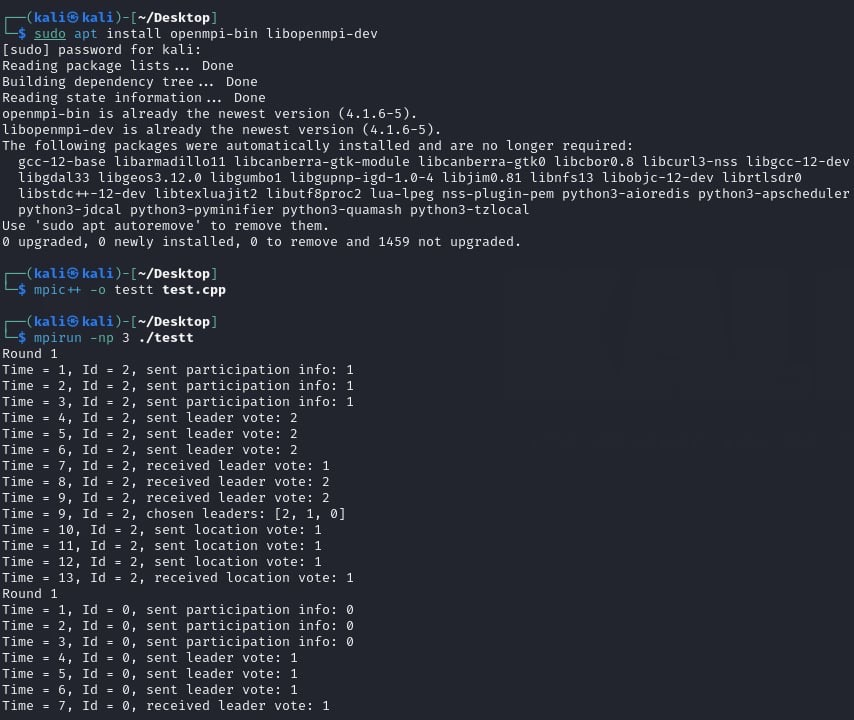
\includegraphics[width=0.8\textwidth]{Deploy_MPI.png}
  \caption{Result 1: Deploy MPI.}
\end{figure}

\begin{figure}[h]
  \centering
  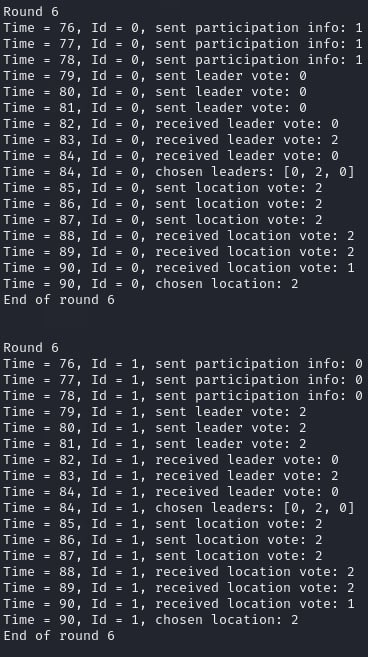
\includegraphics[width=0.8\textwidth]{Result_MPI.png}
  \caption{Result 2: Result of MPI.}
\end{figure}

\end{document}
